%!TEX root = ./main.tex

\section{Local methods for design \& verification}\label{section:local_methods}

To design complex systems, engineers in many fields use computer-aided tools to boost their productivity. Mechanical engineers can use a suite of 3D CAD (computer-aided design) and FEA (finite-element analysis) tools to design structures and understand their performance. Likewise, electrical engineers use electronic design automation tools, including hardware description languages like Verilog, to design and analyze large-scale, reliable, and yet highly complex integrated circuits. Sadly, when it comes to designing autonomous systems and robots, engineers often take an ad-hoc approach, relying heavily on experience and tedious parameter tuning.

Two factors have made it difficult to develop automated design tools for robotics. The first is complexity: most robots are composed of many interacting subsystems. Although some tools may aid in designing certain subsystems (e.g. Simulink for controllers, SolidWorks or CATIA for hardware, custom software for training perception systems), these tools cover only a small part of the overall robotics design problem, which includes sensing, actuation, perception, navigation, control, and decision-making subsystems. In addition to being interconnected, these subsystems often have a large number of parameters that require tuning to achieve good performance (neural network-based perception is an extreme example of this trend). Moreover, since few robotic systems are exactly alike, an effective design tool must allow the user to select an appropriate level of abstraction for the problem at hand. As a result, there is a need for flexible computational tools that can help designers optimize complex robotic systems.

The second difficulty is uncertainty. Robots operate in dynamic environments that cannot be fully specified \textit{a priori}, and nonlinear interactions between the robot and its environment can make this uncertainty difficult to quantify. Nevertheless, we must account for this uncertainty during the design process and ensure that our designs perform robustly. The nature of this uncertainty can vary from problem to problem, reiterating the requirement that an automated design tool must be flexible enough to adapt to different robot design problems.

To be successful, an automated robot design tool must address these two challenges (complexity and uncertainty). In addition, just as mechanical and electrical engineers use automated tools to both \textit{design} and \textit{verify} their designs, a robot design tool must enable its user to both design autonomous systems and test the robustness of those designs. In addition, we would also like the ability to close the loop between design and verification, feeding the results of verification back into the design process to make the system more robust (i.e. \textit{verification-guided design}).

In this section, we frame these three tasks as optimization problems in order to develop local optimization-based solution methods. In doing so, we introduce terminology and notation that will be used in the rest of this proposal. Approaching these problems through the lens of optimization is a natural first step, and we will show empirically that it can lead to good results in a number of robotics settings; however, a purely optimization-based mindset has several limitations, which we will discuss at the end of this chapter with an eye towards resolving in the next.

\subsection{Problem statement}

% Math-ify the setting: free parameters, exogenous parameters, simulator, cost function. Maybe a table to summarize the notation.

% Show how that works for the motivating example

At the heart of any design process is the tension between the factors a designer can control and those she cannot. For instance, a designer might be able to choose the locations of sensors and tune controller gains, but she cannot choose the sensor noise or disturbances (e.g. wind) encountered during operation.
Robot design is therefore the process of choosing feasible values for the controllable factors (here referred to as \textit{design parameters}) that achieve good performance despite the influence of uncontrollable factors (\textit{exogenous parameters}).

Of course, this is a deliberately narrow view of engineering design, since it focuses on parameter optimization and ignores important steps like problem formulation and system architecture selection. Our focus on parameter optimization is intentional, as it allows the designer to focus her creative abilities and engineering judgment on the architecture problem, using computational aids as interactive tools in a larger design process \cite{sharpe_thesis,cascaval2021differentiable}. This focus is common in design optimization (e.g. aircraft design in~\cite{sharpe_thesis} and 3D CAD optimization in~\cite{cascaval2021differentiable}). Formally, we can model the design process as having four components, as illustrated in Fig.~\ref{ch5:fig:block_diagram}.

\paragraph{Design parameters} The system designer has the ability to tune certain continuous free parameters $x \in \cX \subseteq \R^n$; e.g., control gains or the positions of nodes in a sensor network. We assume that constraints on the design parameters are captured in the structure of $\cX$.

\paragraph{Exogenous parameters} Some factors are beyond the designer's control, such as wind speeds or sensor noise. We model these effects as continuous paramaters $y \in \cY \subseteq \R^m$, which we assume follow some prior likelihood $p_{0, y}$ supported on $\cY$. In this section, we assume no knowledge of $p_{0, y}$ other than the ability to sample from it, but we will revisit this assumption in subsequent chapters to see what insights can be gained from the structure of $p_{0, y}$.

\paragraph{Simulator} Given particular choices for $x$ and $y$, the system's state $s \in \mathcal{S}$ evolves in discrete time according to a known simulator $S : \cX \times \cY \mapsto \mathcal{S}^T$. This simulator describes the system's behavior over a finite horizon $T$ as a trace of states $s_1, \ldots, s_T$. We assume that $S$ is deterministic; randomness must be ``imported'' via the exogenous parameters.

\paragraph{Cost} We assume access to a function $J: \mathcal{S}^T \mapsto \mathbb{R}$ mapping system behaviors (i.e. a trace of states) to a scalar performance metric that the designer seeks to minimize.

\ \\

\begin{figure}[tb]
    \centering
    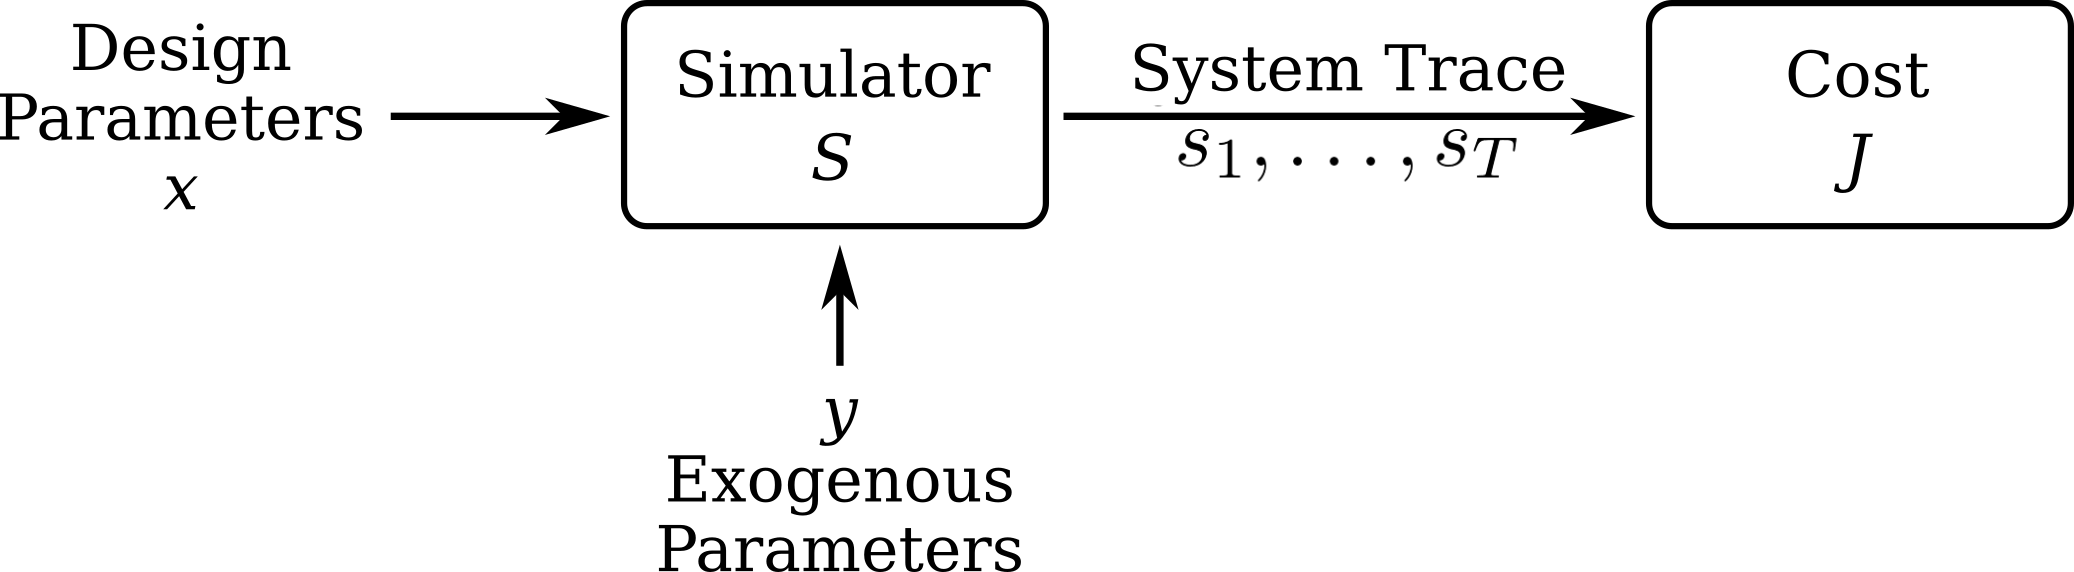
\includegraphics[width=0.6\linewidth]{images/ch5/block_diagram.png}
    \caption{A high-level model of the design and verification problem for an autonomous system. Design optimization involves finding a set of design parameters so that the simulated cost is minimized, while verification involves understanding how changes in the exogenous parameters affect the simulated cost.}
    \label{ch5:fig:block_diagram}
\end{figure}

In this context, we can formalize the design, verification, and verification-guided design tasks as optimization problems. For the time being, we take a worst-case approach to verification, but we will revisit this in Section~\ref{section:global_methods}.

\begin{align}
    \textit{Design: }                     & x = \argmin_{x \in \cX} \expectation_{y \sim \cY}\left[ J(S(x, y)) \right] \label{ch5:eq:design}     \\
    \textit{Verification: }               & y = \argmin_{y \in \cY} J(S(x, y))    \label{ch5:eq:verification}                                    \\
    \textit{Verification-guided design: } & x = \argmin_{x \in \cX} \max_{y \in \cY} J(S(x, y)) \label{ch5:eq:verification_guided_design_minmax}
\end{align}

These problems have been studied in various forms throughout the prior literature, but previous works tend to either use sample-inneficient black-box optimization techniques~\cite{corsoAdaptiveStressTesting2019,corsoSurveyAlgorithmsBlackBox2021a,dingLearningCollideAdaptive2020a,wangAdvSimGeneratingSafetyCritical2021a} or focus on developing application-specific algorithms for certain cases where gradients can be derived~\cite{Schulz_robogami,du2016computational,du2021underwater,ma2021diffaqua,xu_uav_controllers}. The first contribution in this chapter is to expand on these application-specific works to demonstrate how automatic differentiation enables us to easily apply gradient-based optimization methods to solve the design and verification problems.

Unfortunately, while simply feeding AD-derived gradients into off-the-shelf optimizers is a natural (and often effective) first step, it provides few assurances of that our optimized designs will be robust, and does little to connect the results of verification back into the design process. The second contribution in this chapter is to close this gap by developing a framework that uses AD-derived gradients to accelerate adversarial testing.

This chapter presents work published in RSS 2022~\cite{dawsonCertifiableRobotDesign2022a} and IROS 2022~\cite{dawsonRobustCounterexampleguidedOptimization2022}. In the interest of brevity, we defer implementation details to the appendix and focus here on the key ideas, results, and limitations.

\subsection{Efficient design optimization using differentiable simulation}

A natural first instinct when presented with gradients from an automatic differentiation system is to apply a gradient-based optimizer to find low-cost design parameters. This approach is simple (relying on pre-existing optimization methods), flexible (using general-purpose AD libraries to model subsystems with varying levels of abstraction), and efficient (making use of gradients to accelerate the search for high-performing designs).

Although it is possible to directly optimize the objective in~\eqref{ch5:eq:design} to find low-cost design parameters, in many practical use-cases we are interested in designs that are not only low-cost but robust to variation in $y$, which we can encode by regularizing the objective with respect to the variance of the cost:
%
\begin{subequations}\label{ch5:eq:design_optimization_nlp_generic}
    \begin{align}
        \min_{x \in \cX} & \quad \expectation_{y \sim \cY} \Big[ J\circ S\pn{x, y} \Big] + \lambda \rm{Var}_{y\sim\cY}\Big[ J\circ S\pn{x, y} \Big] \label{ch5:eq:design_optimization_objective_generic}
    \end{align}
\end{subequations}
%
To yield a tractable problem, we replace the expectation and variance with unbiased estimates over $N$ samples $y_i \sim \cY, i=1,\ldots,N$.
%
\begin{subequations}\label{ch5:eq:design_optimization_nlp}
    \begin{align}
        \min_{x \in \cX} & \quad \frac{1}{N}\sum_{i=1}^{N} \Big[J\circ S\pn{x, y_i}\Big] + \lambda \left[ \frac{\sum_{i=1}^N \pn{J\circ S\pn{x, y_i}}^2}{N-1} - \frac{\pn{\sum_{i=1}^N J\circ S\pn{x, y_i}}^2}{(N-1)N} \right] \label{ch5:eq:design_optimization_objective}
    \end{align}
\end{subequations}

Since computing this objective requires multiple calls to the simulator $S$, approximating the gradients of~\eqref{ch5:eq:design_optimization_objective} using finite-differences or stochastic multi-sample estimators would incur a large computational cost (requiring $O(N\dim{x})$ calls to $S$). Fortunately, backwards-mode AD allows us to obtain these gradients much more cheaply, with a constant $O(N)$ simulator calls, regardless of the dimension of the search space. On high-dimensional problems, like optimizing a neural network planning system for the multi-robot collaborative manipulation system shown in Fig.~\ref{ch5:fig:mam_hw}, the improved scaling of AD is clearly apparent. In this example, where the cost measures how close the robots were able to maneuver the box to its desired pose (which varies randomly along with uncertain coefficients of friction in the environment), $\dim{x} = 454$ and $N = 512$, so AD requires two orders of magnitude fewer simulator evaluations than a finite-difference scheme.

This improved scaling can be seen empirically if we compare the time required to run L-BFSG-B (a quasi-Newton first-order optimizer) until convergence using both AD-derived and finite-difference gradients. Fig.~\ref{ch5:fig:ablation} shows that although both methods achieve a similar optimal cost, AD-based optimization runs 20x faster (even after accounting for the additional computational overhead of backwards-mode AD).

\begin{figure}[tb]
    \centering
    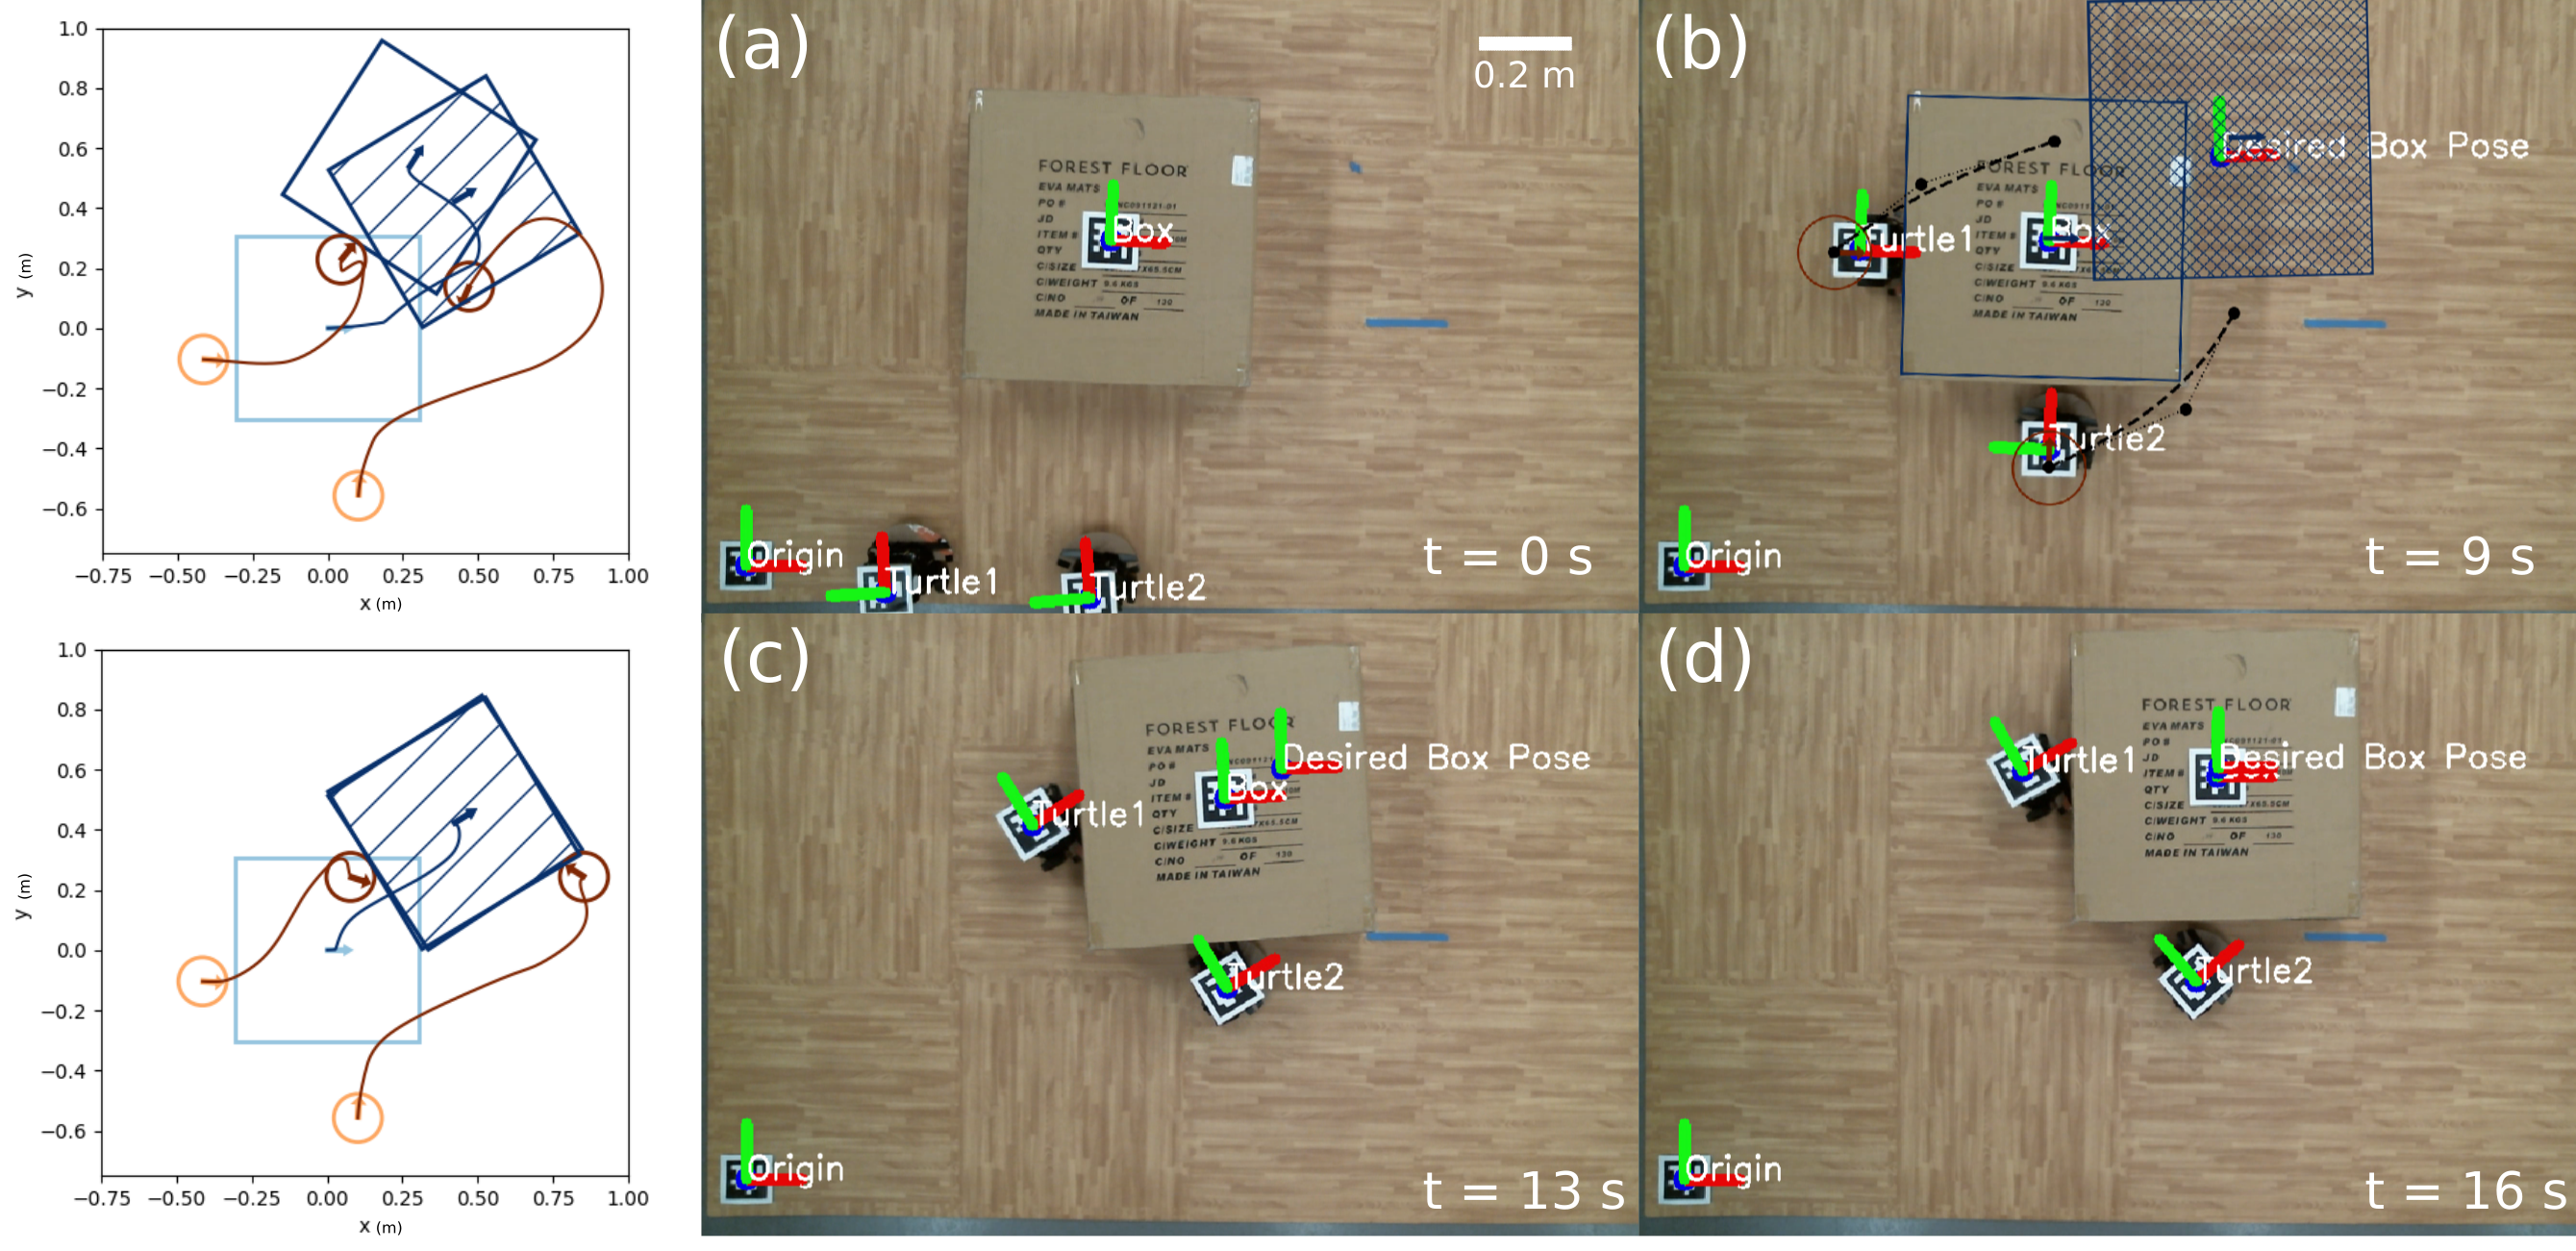
\includegraphics[width=\linewidth]{images/ch5/mam_composite_w_sim.png}
    \caption{Left: Initial (top) and optimized (bottom) manipulation strategies in simulation (light/dark colors indicate initial/final positions, stripes indicate desired position). Right: Optimized manipulation strategy deployed in hardware (video included in the supplementary materials). (a) The robots first move to positions around the box. (b) Using the optimized neural network, the robots plan a cubic spline trajectory pushing the box to its desired location. (c-d) The robots execute the plan by tracking that trajectory.}
    \label{ch5:fig:mam_hw}
\end{figure}

\begin{figure}[t]
    \centering
    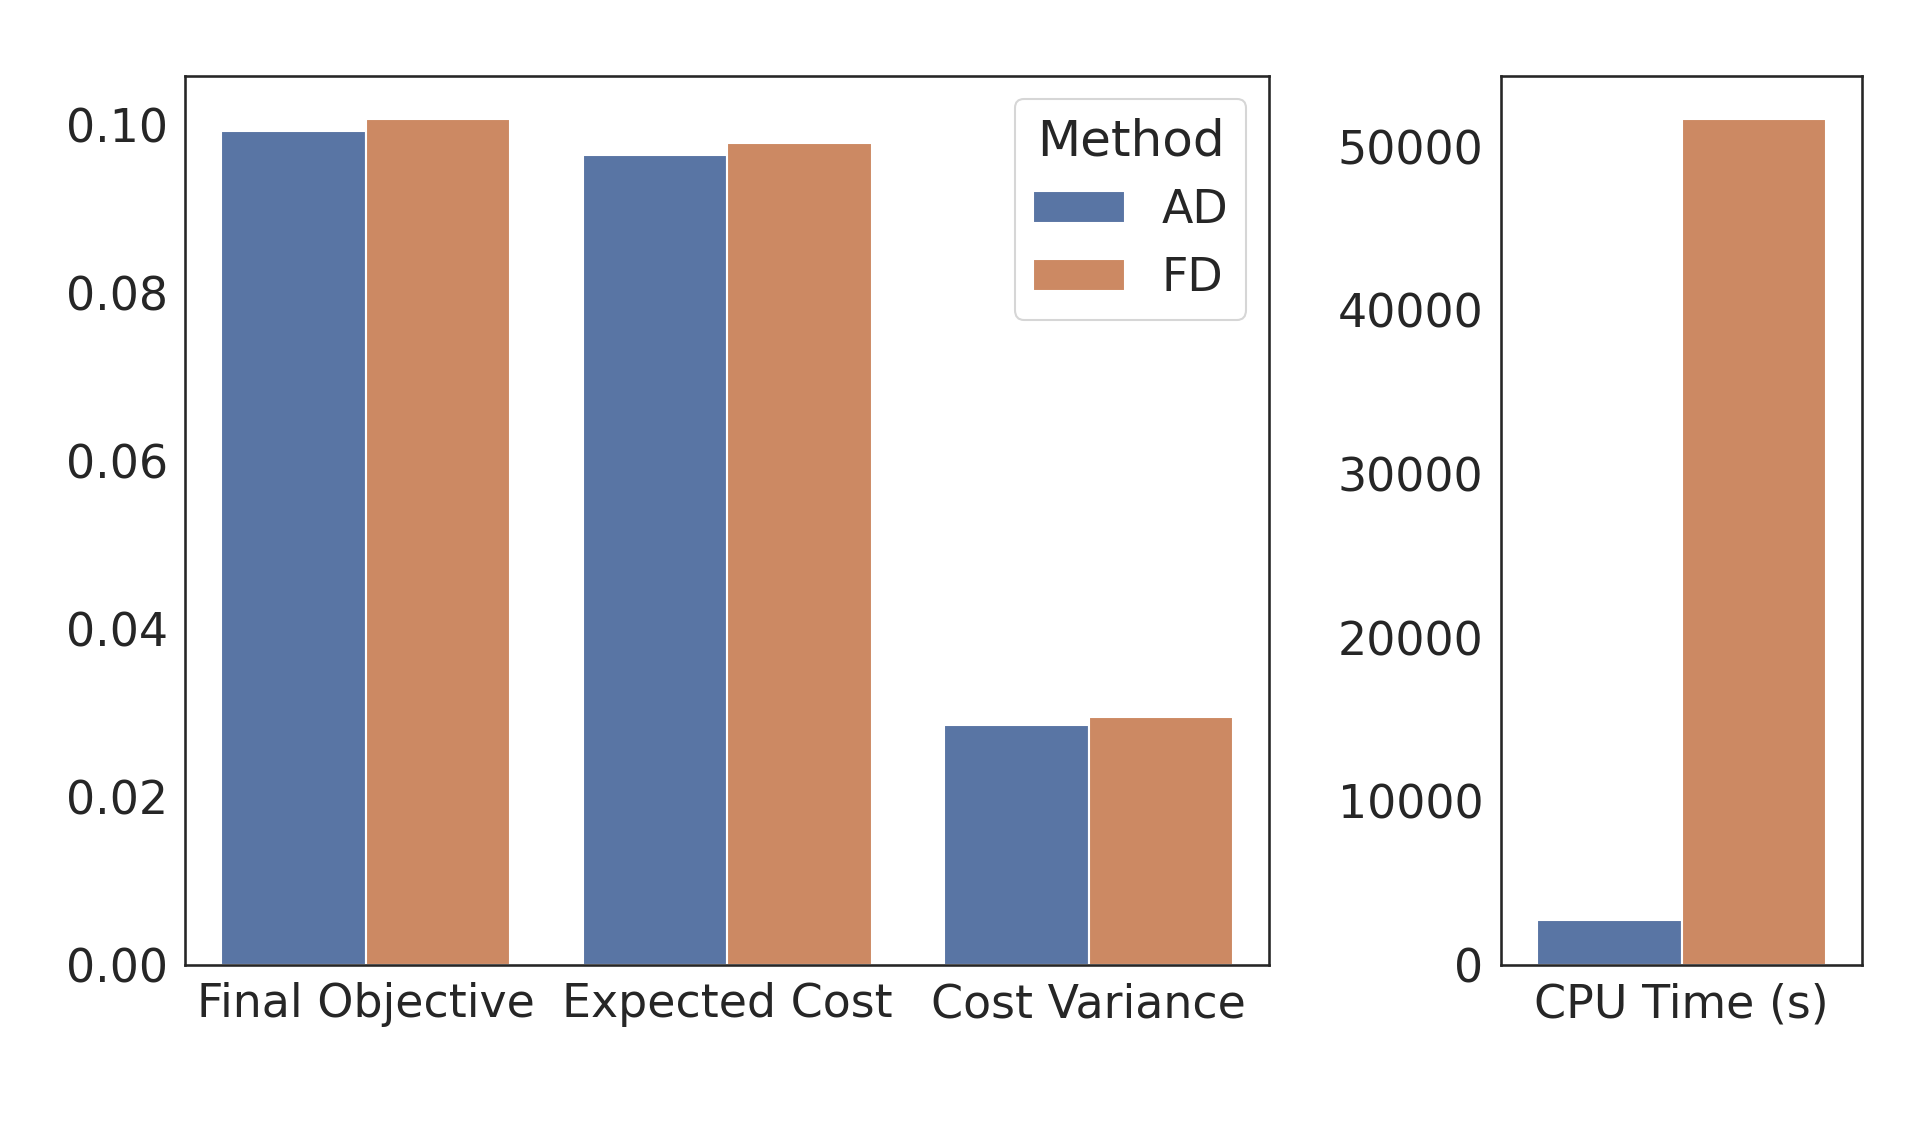
\includegraphics[width=0.7\linewidth]{images/ch5/mam_ablation_ad_fd.png}
    \caption{Improvement of automatic differentiation (AD) over finite differences (FD) on the multi-agent manipulation case study shown in Fig.~\ref{ch5:fig:mam_hw}.}
    \label{ch5:fig:ablation}
\end{figure}

\subsection{Local adversarial testing for verification-guided design}

The results in the previous section show how we can use AD for efficient and robust gradient-based optimization; however, the computational expense of averaging over exogenous parameters makes it difficult to scale to larger systems that may be more difficult to simulate. In addition, in many safety-critical contexts we are interested in verifying not only the average-case but the worst-case behavior.

These difficulties motivate the next contribution of this chapter, where we introduce an adversarial optimization approach to solving the min/max problem~\eqref{ch5:eq:verification_guided_design_minmax}. Of course, solving~\eqref{ch5:eq:verification_guided_design_minmax} to global optimality in the general nonlinear case is intractable. Instead, we take advantage of this game structure to design an iterative algorithm to find the \textit{generalized Nash equilibrium}: the design parameters $x$ and corresponding $y$ such that neither the planner nor the adversary have an incentive to change their choice~\cite{facchineiGeneralizedNashEquilibrium2007a}.

To solve for such an equilibrium, a common strategy is the family of nonlinear Gauss-Seidel-type methods. These methods solve max-min problems like~\eqref{ch5:eq:verification_guided_design_minmax} by alternating between $x$ and $y$, tuning one set of parameters while keeping the others constant; i.e. alternating between the two optimization problems:
\begin{subequations}
    \begin{align}\label{ch5:eq:gauss_seidel}
        x^* & = \argmin_x J(x, y^*) \\
        y^* & = \argmax_y J(x^*, y)
    \end{align}
\end{subequations}
Although these methods are not guaranteed to converge, it is known that if they do, then the convergence point $(x^*, y^*)$ is a Nash equilibrium~\cite{facchineiGeneralizedNashEquilibrium2007a}.

A risk of applying such a simple alternating scheme is that the nonlinear optimization for both $x$ and $y$ can easily get caught in local minima, which increases the risk of ``overfitting'' the design to a particular value of $y^*$. To mitigate the risk of overfitting and improve the robustness of our optimized design, we extend the standard Gauss-Seidel method with two ideas from the machine learning and optimization literature. First, we take inspiration from the success of domain randomization in robust machine learning~\cite{tobinDomainRandomizationTransferring2017}: instead of optimizing $x$ with respect to a single fixed $y^*$, we can maintain a dataset $\cY_N = \set{y_i}_{i=1,\ldots,N}$ and optimize the performance of $x$ across all of these samples:
\begin{subequations}
    \begin{align}\label{ch5:eq:gauss_seidel_domain_randomization}
        x^* & = \argmin_x \mathbb{E}_{\cY_N} \left[ J(x, y_i) \right] \\
        y^* & = \argmax_y J(x^*, y)
    \end{align}
\end{subequations}

This domain-randomized objective is similar to that used in the previous section and has the potential to improve the robustness of the resulting equilibria, but it is relatively sample inefficient; it may require a large number of random samples $y_i$ to cover the range of possible system behaviors. To address this sample inefficiency, we take inspiration from a second idea in the optimization and learning literature: learning from counterexamples~\cite{changNeuralLyapunovControl2019}. The key insight here is that we can do better than simply randomly sampling $y_i$; we can use the values of $y^*$ found during successive iterations of the Gauss-Seidel process as high-quality counterexamples to guide the optimization of $x$. This insight results in our counterexample-guided Gauss-Seidel optimization method, which is outlined in pseudocode in Algorithm~\ref{ch5:alg:cg_gs}.

Our algorithm proceeds as follows. We begin by initializing the dataset with $N_0$ i.i.d. examples $y_i$, then we alternate between solving the two optimization problems in~\eqref{ch5:eq:gauss_seidel_domain_randomization}. At each iteration, we add our current estimate of the adversary's best response $y^*$ to the dataset, and we stop either when the algorithm reaches a fixed point (the adversary's best response after solving~\eqref{ch5:eq:gauss_seidel_domain_randomization} is the same as the best response from the previous round) or when a maximum number of iterations is reached. As we will show in our experiments in the next section, this counterexample-guided optimization achieves a higher sample efficiency than simple domain randomization ---  it finds designs that are more robust to adversarial disturbance while considering a much smaller dataset. Although our use of nonlinear optimization means that our algorithm is not complete, we find empirically that it succeeds in finding a satisfactory design in the large majority of cases.

It is important to note that this algorithm is enabled by automatic differentiation; without access to the gradients of $J$ it would be much more difficult to solve the subproblems in lines~\ref{ch5:alg:opt_theta} and~\ref{ch5:alg:opt_chi} of Algorithm~\ref{ch5:alg:cg_gs}. We are not aware of any approaches that make use of automatically-derived gradients with respect to disturbance parameters for adversarial verification-guided optimization.

\begin{algorithm}
    \caption{Counterexample-guided Gauss-Seidel method for solving robust planning problems}\label{ch5:alg:cg_gs}
    \DontPrintSemicolon
    \KwInput{Starting dataset size $N_0$\\\phantom{Input: } Maximum number of iterations $M$}
    \KwOutput{Optimized design parameters $x^*$\\\phantom{Output: } Dataset of counterexamples $\set{y^*}$}
    $\set{y^*} \gets $ $N_0$ examples $y_i \in \cY$ sampled uniformly i.i.d.\;
    $y^*_{prev} \gets \varnothing$\;
    \For{$i \in \set{1, \ldots, M}$}
    {
        $x^* = \argmin_x \mathbb{E}_{\cY_N} \left[ J(x, y_i) \right] \label{ch5:alg:opt_theta}$ \;
        $y^* = \argmax_y J(x^*, y)$ \label{ch5:alg:opt_chi} \;
        \If{$y^* = y^*_{prev}$}{\Break}
        $y^*_{prev} \gets y^*$\;
        Append $y^*$ to $\set{y^*}$\;
    }
    \KwRet{$x^*$, $\set{y^*}$}
\end{algorithm}

To validate this approach, we can use two case studies involving planning and control for the satellite rendezvous problem posed in~\cite{jewisonSpacecraftBenchmarkProblem2016}. We define this planning problem using signal temporal logic (STL), which provide a formal language for capturing complex behavioral requirements and specifying how a robot behaves over time. For a brief introduction to the syntax and semantics of STL, see~\cite{dawsonRobustCounterexampleguidedOptimization2022}. By restricting this case study to focus on planning, we are able to benchmark against state-of-the-art planning algorithms to show the robustness and scalability benefits of our adversarial optimization-based approach. We implement a smooth differentiable version of STL following the approach in~\cite{leungBackPropagationSignalTemporal2021,pantSmoothOperatorControl2017}.

In this satellite rendezvous problem, the goal is to maneuver a chaser satellite to catch a target satellite. In this setting, we construct STL specifications for two rendezvous missions: a simple low-speed rendezvous and a more complex loiter-then-rendezvous mission, illustrated in Fig.~\ref{ch5:fig:mission_specs}. The STL specifications for each mission, $\psi_1$ and $\psi_2$, are given formally as:
\begin{align*}
    \psi_1                   & = \psi_\text{reach target} \wedge \psi_\text{speed limit}                           \\
    \psi_2                   & = \psi_\text{reach target} \wedge \psi_\text{speed limit} \wedge \psi_\text{loiter} \\
    \psi_\text{reach target} & = \eventually \pn{r \leq 0.1}                                                       \\
    \psi_\text{speed limit}  & = \pn{r \geq 2.0} \until\ \always \pn{v \leq 0.1}                                   \\
    \psi_\text{loiter}       & = \eventually \always_{[0, T_{obs}]} \pn{2.0 \leq r \wedge r \leq 3.0}
\end{align*}
where $r = \sqrt{p_x^2 + p_y^2 + p_z^2}$ and $v = \sqrt{v_x^2 + v_y^2 + v_z^2}$.

These formulae can be read as follows: $\psi_\text{reach target}$ specifies that ``the chaser eventually comes within \SI{0.1}{m} of the target'', $\psi_\text{speed limit}$ specifies that ``once the chaser is within \SI{2.0}{m} of the target, its speed cannot exceed \SI{0.1}{m/s}'', and $\psi_\text{loiter}$ specifies that ``at some point during the mission, the chaser should spend $T_{obs}$ seconds between 2--\SI{3}{m} away from the target''. The two missions are build from these three building blocks: mission 1 includes the ``reach target'' and ``speed limit'' requirement, while mission 2 includes all three requirements.

For each mission, the design parameters $x$ include both state/input waypoints along a planned trajectory and the feedback gains used to track that trajectory, and the exogenous parameters $y$ represent bounded uncertainty in the initial state of the chaser ($p_x(0), p_y(0) \in [10, 13]$, $p_z(0) \in [-3, 3]$, $v_x(0), v_y(0), v_z(0) \in [-1, 1]$). We use a \SI{200}{s}-long simulation with a \SI{2}{s} timestep for both missions, and $T_{obs} = \SI{10}{s}$.

\begin{figure}[t]
    \centering
    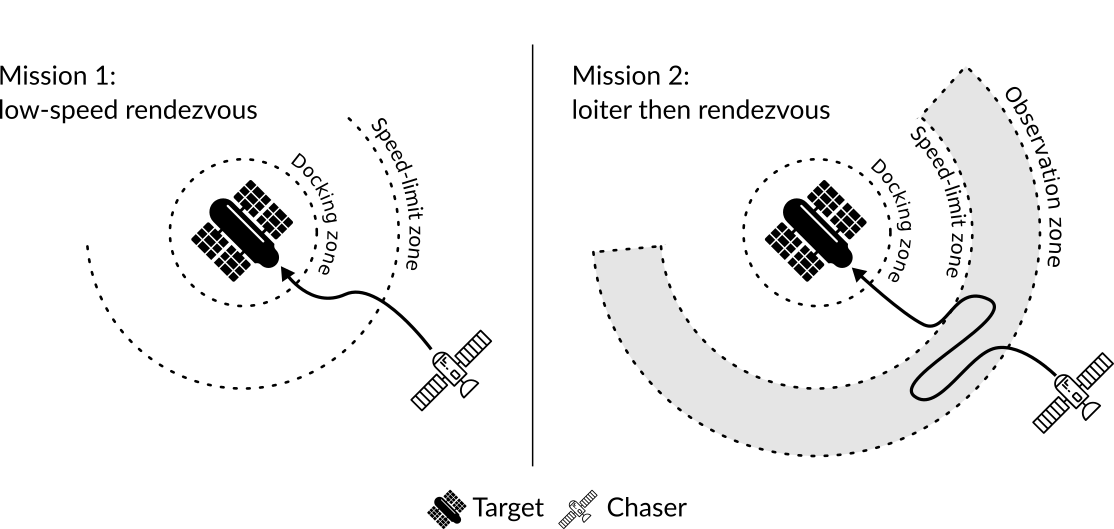
\includegraphics[width=0.7\linewidth]{images/ch5/satellite_missions.png}
    \caption{Two satellite rendezvous missions used to test our adversarial optimization framework. In the first mission, the chaser satellite must eventually reach the target while respecting a maximum speed constraint in the region immediately around the target. In the second mission, the chaser must still reach the target and obey the speed limit, but it must also loiter in an observation region for some minimum time before approaching. The first mission requires an STL formula with three predicates and three temporal operators, while the second mission requires five predicates and five temporal operators.}
    \label{ch5:fig:mission_specs}
\end{figure}

For each mission $i=1, 2$, we define a cost function as $J_i = -\rho_i + \lambda I$, where $\rho_i = \rho(\psi_i, S(x, y), 0)$ is the STL robustness margin at the start of the trajectory (i.e. how satisfied/unsatisfied the requirements are), $I$ is the total impulse required to execute the maneuver (in Newton-seconds), and $\lambda = 5\times10^{-5}$. By applying our iterative counterexample-guided optimization strategy to this problem, we find the optimized trajectories for mission 1 and 2 shown in Fig.~\ref{ch5:fig:mission_trajs} along with the worst-case $y$. In these examples, we use $N_0=8$ initial examples and $M=10$ maximum rounds, but the algorithm converges in less than 10 rounds in all trials. In both missions, our approach reliably finds a solution that remains feasible despite worst-case variation in the exogenous parameters, achieving a positive STL robustness margin in $>90\%$ of trials in each case. Our counterexample-guided approach requires an average of \SI{53.7}{s} to solve mission 1 and \SI{194.2}{s} to solve mission 2 (averaged across 50 trials).

\begin{figure}[t]
    \centering
    \begin{subfigure}[t]{0.4\linewidth}
        \centering
        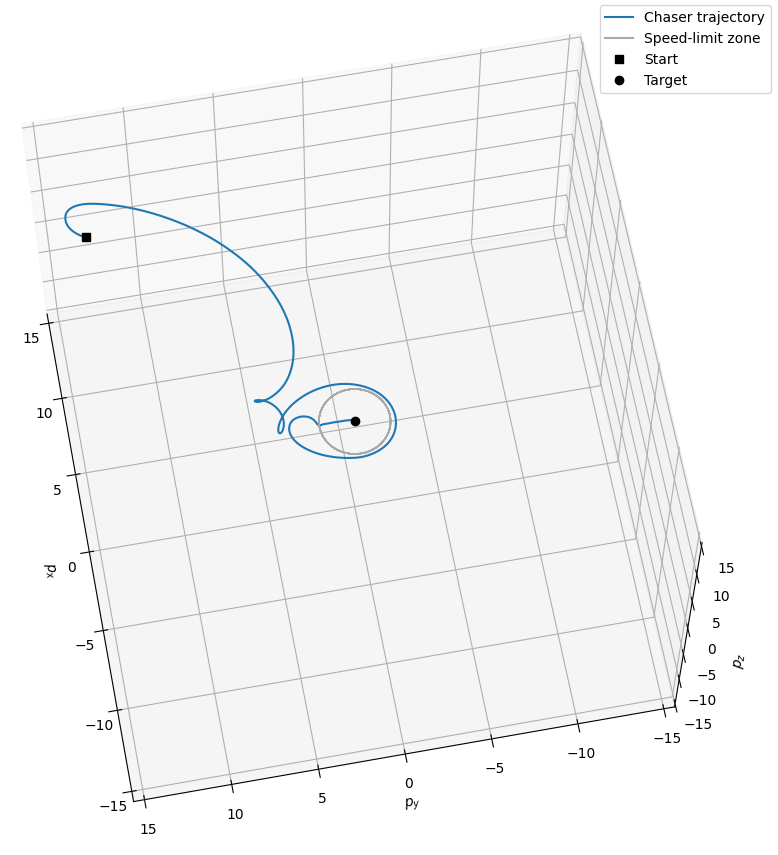
\includegraphics[width=\linewidth]{images/ch5/satellite_mission1_traj.png}
        \caption{Mission 1}
    \end{subfigure}
    \begin{subfigure}[t]{0.4\linewidth}
        \centering
        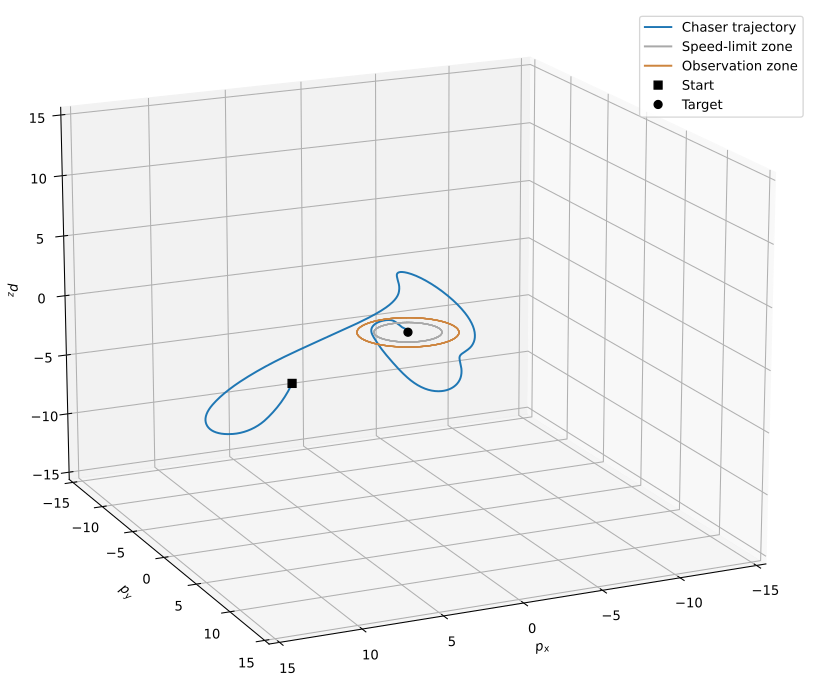
\includegraphics[width=\linewidth]{images/ch5/satellite_mission2_traj.png}
        \caption{Mission 2}
    \end{subfigure}%
    \caption{(a) The optimized trajectory found using our counterexample-guided optimization strategy for mission 1 (rendezvous with speed constraint). The chaser satellite only enters the speed-limit zone once it has slowed down sufficiently. (b) The optimized trajectory for mission 2 (loiter then rendezvous with speed constraint), satisfying the additional mission requirement of spending time in the observation region before approaching the target.}
    \label{ch5:fig:mission_trajs}
\end{figure}

To quantify the advantage of our AD-enabled adversarial optimization method relative to the state-of-the-art, there are two salient comparisons. First, what advantage does adversarial optimization have relative to domain randomization? Second, since we are solving a specialized motion planning problem, how does our method compare against application-specific solvers for this STL planning problem?

To answer the first question, we compare our adversarial method with non-adversarial optimization with domain randomization with 64 and 32 samples, as well as non-adversarial optimization without any domain randomization (1 sample). To answer the second question, we compare with a mixed-integer programming (MIP) approach to solving STL planning problems~\cite{sunMultiagentMotionPlanning2022}. The results of this comparison are shown in~\ref{ch5:fig:stl_comparisons}. All experiments were run on a laptop computer with \SI{8}{GB} RAM and a \SI{1.8}{GHz} 8-core processor, with no GPU, and results are averaged over 50 random seeds.

We find that our method is consistently more robust than prior methods; in the first mission, it satisfies the STL specification in all but 3 trials, despite adversarial disturbances. For comparison, the next-best method (domain randomization with 64 samples) failed to solve the first mission in 14 out of 50 trials and took more than twice as long on average to find a plan (\SI{114.3}{s} as opposed to \SI{53.7}{s} for our method). This advantage is due to the quality of the examples used during optimization; instead of 64 random samples, our method uses 8 initial random samples and between 1 and 4 counterexamples (median 2) representing worst-case variation in $y$, making our method much more sample-efficient. This pattern also holds on the second mission, where 64-sample domain randomization takes more than twice as long as our method and fails to satisfy the STL specification in 17 out of 50 trials (compared to only 4 failures for our method). Our method required a median of 2 counterexamples in addition to the 8 initial examples to solve the second mission (the slowest trial required 7 additional examples).

We also find that our method finds more robust solutions than the MIP method, since MIP cannot tractably consider variation in $y$ (the MIP method is also unable to find a feasible solution within \SI{500}{s} in 16 out of 50 trials). MIP's performance also suffers due to discretization error, since we were forced to discretize the continuous-time dynamics with relatively few knot points (one every \SI{2}{s}) to yield a tractable MIP optimization problem.


\begin{figure}[t]
    \centering
    \begin{subfigure}[t]{0.45\linewidth}
        \centering
        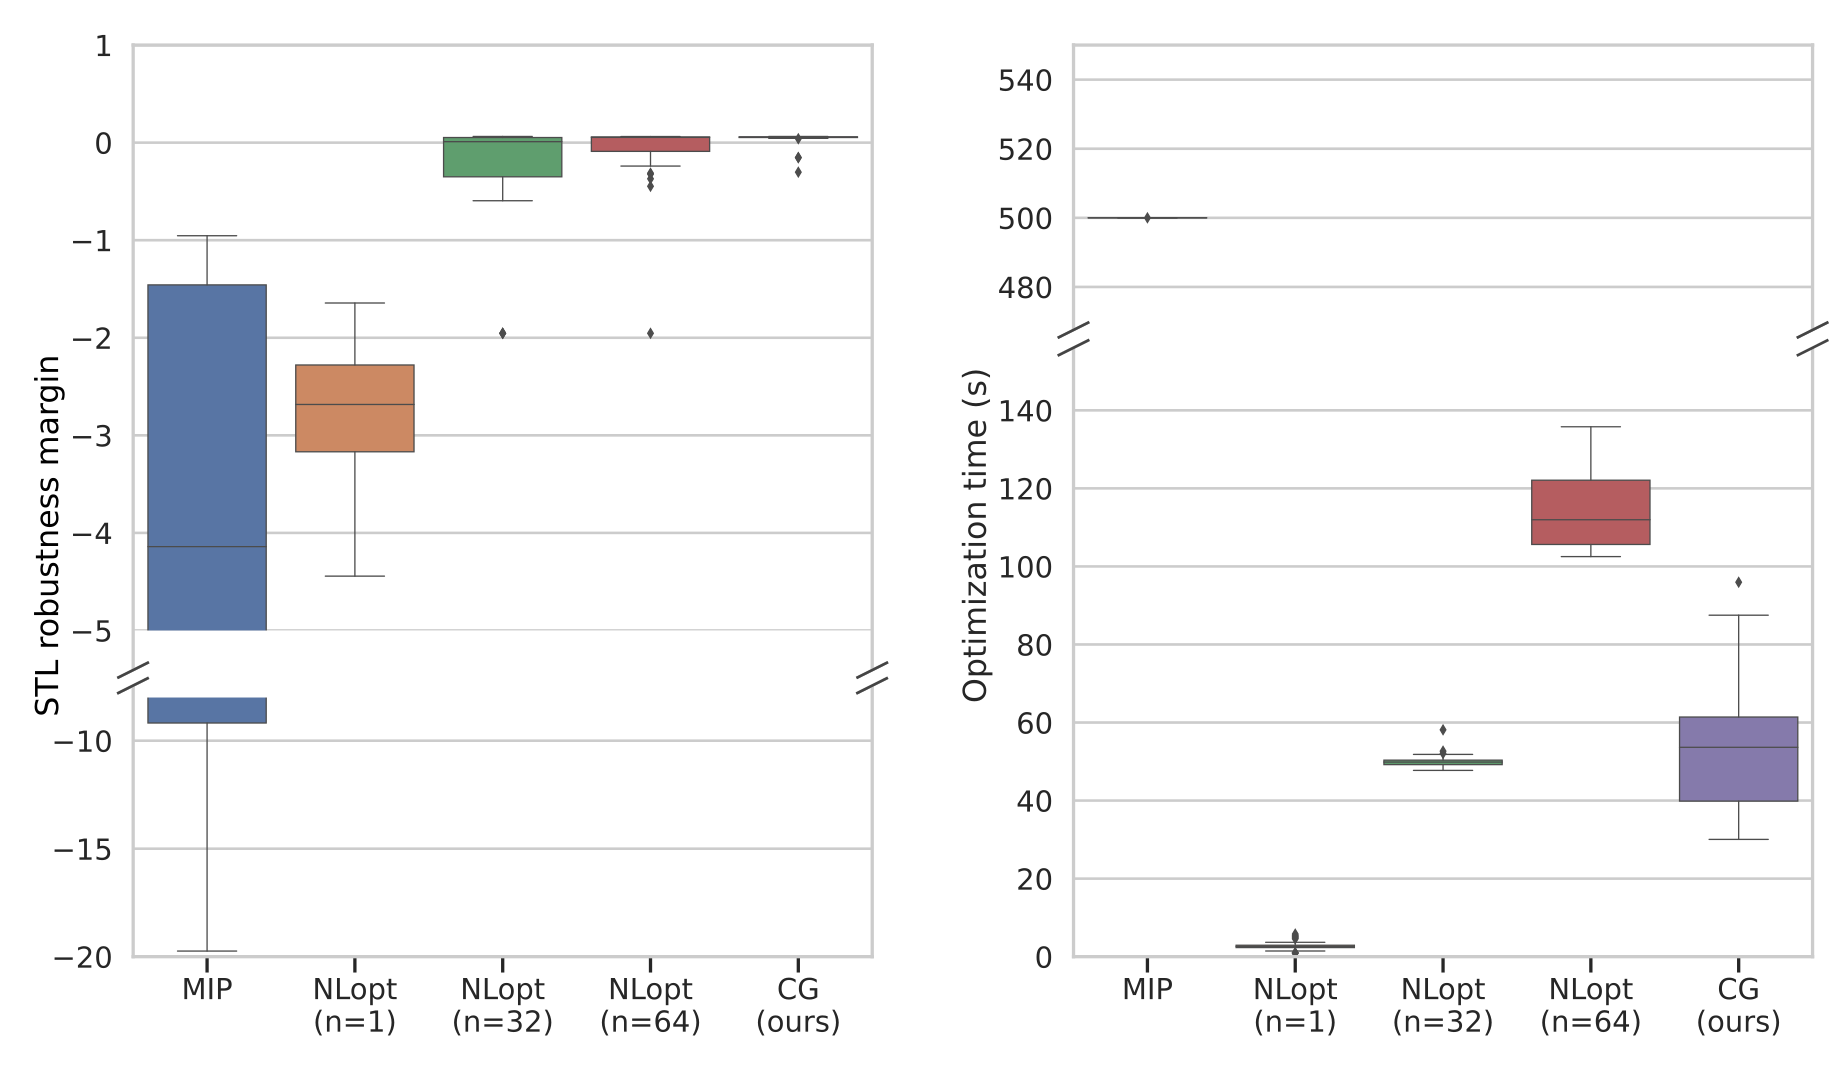
\includegraphics[width=\linewidth]{images/ch5/mission_1_comparison.png}
        \caption{Mission 1}
    \end{subfigure}
    \begin{subfigure}[t]{0.45\linewidth}
        \centering
        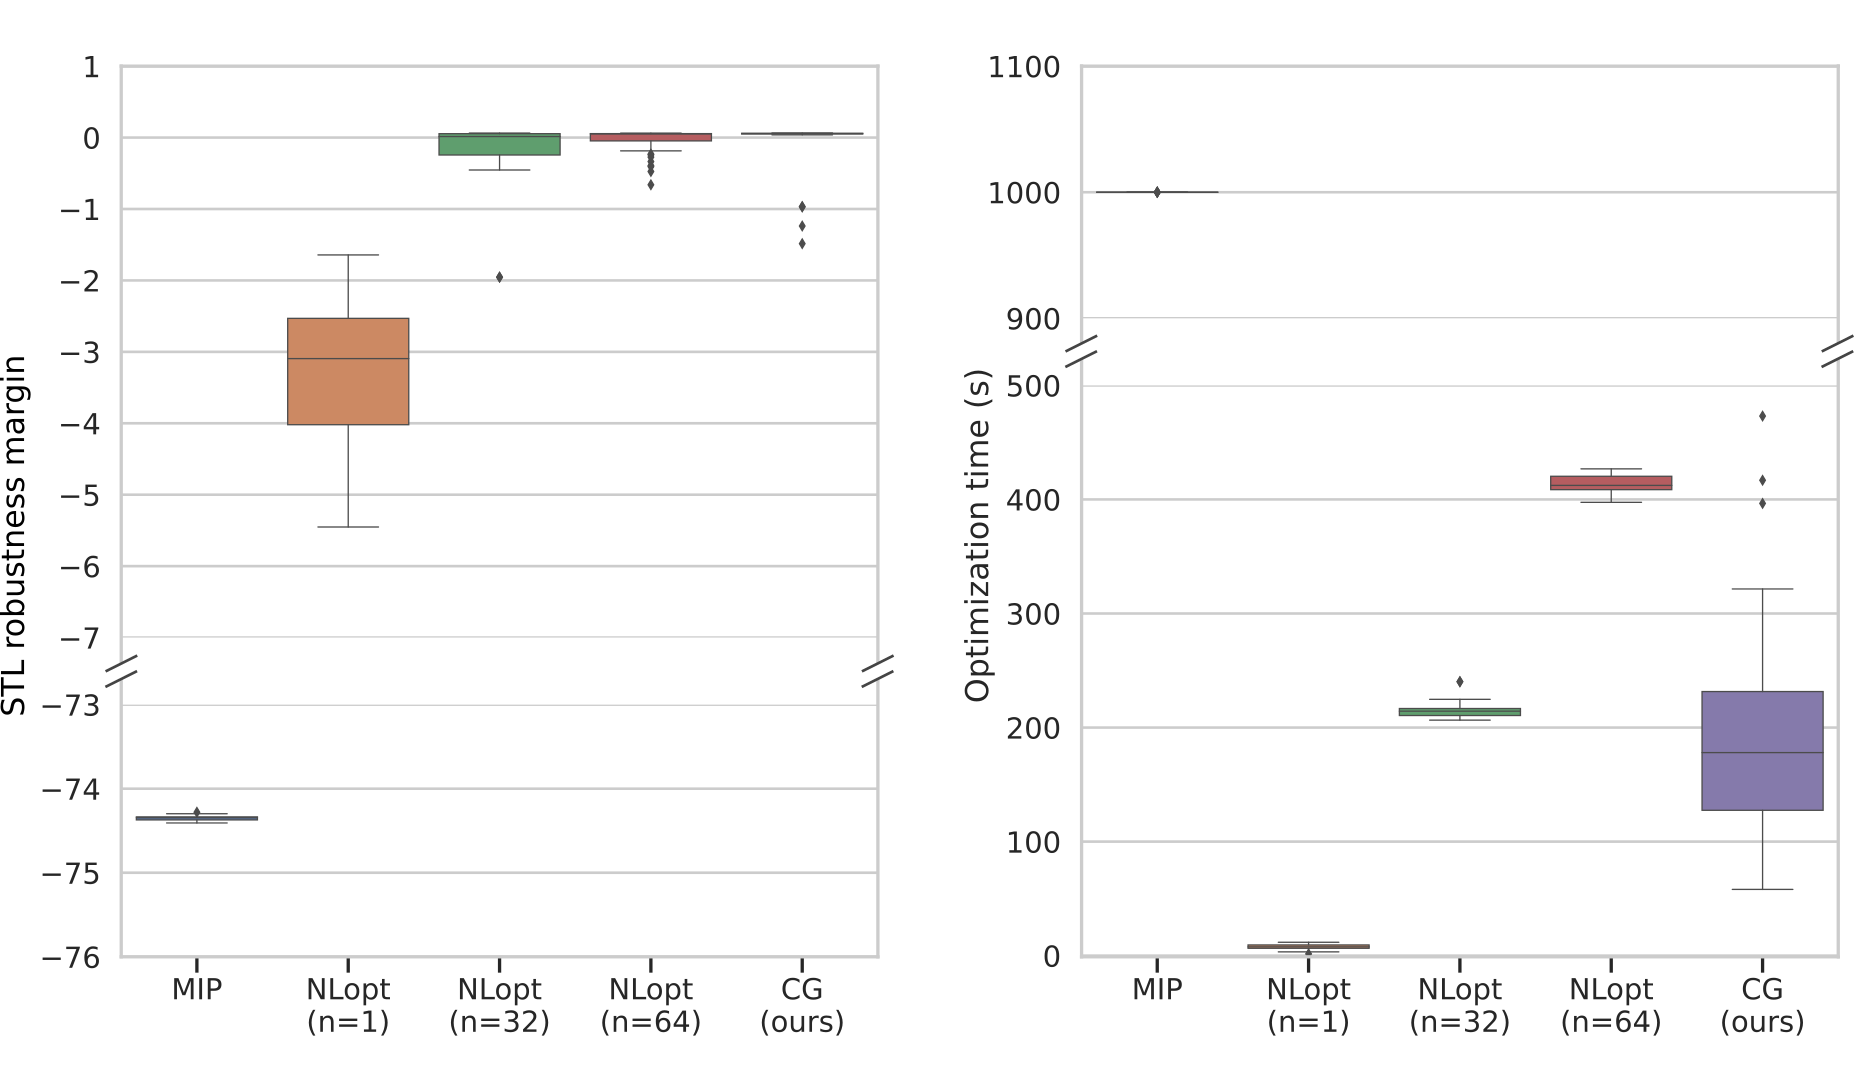
\includegraphics[width=\linewidth]{images/ch5/mission_2_comparison.png}
        \caption{Mission 2}
    \end{subfigure}%
    \caption{Comparison of different STL planning methods on mission 1 (a) and 2 (b), averaged over 50 random seeds. (left subfigures) The robustness margin $\rho(\psi_1)$ computed for the optimized design parameters and worst-case exogenous parameters. (right subfigures) The planning time required by each method. Our method (CG) achieves much higher robustness than all other methods (satisfying the STL specification despite adversarial perturbations in all but 3 instances) and runs twice as fast as the next-most-robust method.}
    \label{ch5:fig:stl_comparisons}
\end{figure}

\subsection{Discussion \& Limitations}

In this chapter, I have presented my previous work on auto-diff-enabled design optimization and verification, with three key takeaways. The first two takeaways are technical and regard the utility of AD for design optimization and verification. First: AD enables a flexible, general-purpose framework for optimizing and verifying a wide-range of robotics problems, with support for multiple interacting subsystems, rich dynamics, and complex task specifications. Second: the use of gradients from AD enables solution methods (such as variance regularization and adversarial optimization) that would be much more computationally expensive if these gradients had to be estimated by other means. The final takeaway is agnostic to the use of AD and concerns how using adversarial optimization can improve both the robustness and the sample efficiency of design optimization (relative to domain randomization).

The main limitation of the work presented in this chapter is its reliance on local gradient-based optimization. As a result, there is still a need for algorithms that take a more global perspective, particularly for verification, which we will introduce in the next chapter.

% Advantages of the differentiable simulation perspective

% Connection to how it can impact working engineers

% Limitations of the local perspective, set up the next section
